\section{Lernen von Graphen}

\subsection{Knotenauswahl}

\begin{itemize}
  \item Auswahl an Knoten, für die ein Receptive Field erstellt werden soll
  \item Sortierung soll dem Verfahren von Bildern nahekommen, d.h. Knoten mit ähnlichen strukturellen Merkmalen sollen auch in der Vektorrepräsentation nah beieinanderliegen
  \item Graph-Beschreibung $l$ – \underline{Metriken}:
  \begin{itemize}
    \item \textbf{Betweenness centrality}:
      \begin{itemize}
        \item $g(v) = \sum_{s \neq v \neq t} \frac{\sigma_{st}(v)}{\sigma_{st}}$
        \item $\sigma_{st}$ beschreibt die Anzahl an kürzesten Pfaden von $s$ nach $t$ ist und $\sigma_{st}$ die Anzahl dieser Pfade, die durch $v$ gehen
      \end{itemize}
    \item \textbf{Eigenvector centrality}:
    \begin{itemize}
      \item \emph{Google's PageRank} ist eine Variante der Eigenvector centrality
      \item $G=(V,E)$ mit Adjazenzmatrix $A$, sodass $a_{v,t} = 1$, falls eine Kante von $v$ nach $t$ existiert
      \item \underline{relative Centrality von $v$:} $x_v = \frac{1}{\lambda} \sum_{t \in N(v)} x_t = \frac{1}{\lambda} \sum{t \in G} a_{v,t}x_t$
      \item kann als Eigenwertproblem formuliert werden: $Ax = \lambda x$
      \item zusätzliche Einschränkung: alle Werte des Eigenvektors $x$ sollen nicht-negativ sein $\Rightarrow$ bestimme größten Eigenwert $\lambda$ $\Rightarrow$ eindeutig
    \end{itemize}
    \item \textbf{Degree centrality:}
    \begin{itemize}
      \item Grad der Knoten, d.h.\ Anzahl adjazenter Knoten (\underline{gewichtet:} Auswärtsgrad – Einwärtsgrad)
    \end{itemize}
    \item \textbf{Closeness centrality:}
    \begin{itemize}
      \item durchschnittliche Länge zwischen dem Knoten und allen anderen Knoten
      \item je zentraler ein Knoten ist, umso näher sind alle anderen Knoten
      \item $C(x) = \frac{1}{\sum_y d(y,x)}$
      \item kann sich für gerichtete Graphen stark unterscheiden (hohe Closeness für ausgehende Kanten, geringe Closeness für eingehene Kanten)
    \end{itemize}
    \item \emph{Weisfeiler-Lehman Algorithmus}
    \item \emph{Page-Rank}
  \end{itemize}
  \item \todo{es werden anscheinend mehrere Metriken benutzt, wie werden diese kombiniert?}
  \item eventuell werden diese Metriken garnicht benötigt, da wir ja eine räumliche Struktur unseres Graphen besitzen, dann kann ähnlich von links nach rechts und von oben nach unten analog zu CNNs auf Bildern vorgegangen werden
  \item \underline{Gegeben:} Graph-Beschreibung $l$, Abstand $s$, Anzahl $w$ an Reciptive Fields
\end{itemize}

\begin{enumerate}
  \item sortiere die Knoten auf Basis von $l$
  \item iteriere über die sortierte Knotenmenge mit Abständen $s$, bis $w$ Knoten ausgewählt wurden
  \item werden weniger als $w$ Knoten gefunden, so werden \emph{all-zero} Receptive Fields erstellt und diese angehängt (\emph{padding purposes})
\end{enumerate}

\subsection{Nachbarschaftssuche}

\begin{itemize}
  \item \underline{Bemerkung:} wahrscheinlich falsche Angabe in Algorithmus 2 $\Rightarrow$ $|L| < |V|$, d.h. Abbruch, wenn keine Knoten mehr eingesammelt werden können
  \item \underline{Gegeben:} Knoten $v$, Größe $k$ des Receptive Fields
\end{itemize}

\begin{enumerate}
  \item setze initiale Knotenmenge $N$ auf $v$
  \item wiederhole bis $|N| > k$:
    \begin{enumerate}
      \item berechne für alle Knoten $i$ in $N$ die Nachbarschaften $N_1(i)$ und füge sie zu $N$ hinzu
    \end{enumerate}
\end{enumerate}

\begin{itemize}
  \item \underline{Bemerkungen:}
  \begin{itemize}
    \item im Allgemein gilt $|N| \neq k$
    \item hier wird das Gewicht der Kanten nicht berücksichtigt, man kann den Algorithmus aber dementsprechend verändern (finde die ersten $k$ Knoten, mit dem kürzesten Pfad zu $v$)
    \item $\Rightarrow$ das ist dann wichtig, wenn das Gewicht etwas über die räumliche Anordnung aussagt
  \end{itemize}
\end{itemize}

\subsection{Normalisierung}

\begin{itemize}
  \item Aus einem Nachbarschaftsgraphen soll ein Receptive Field konstruiert werden
  \item \underline{Problem:} Nachbarschaftssuche liefert uns nicht genau $k$ Knoten, sind nicht sortiert
  \item wenn weniger als $k$ Knoten, dann füge \emph{Dummy-Knoten} hinzu
  \item \underline{Vorgehen}:
  \begin{enumerate}
    \item bestimme Distanz zum Wurzelknoten
    \item führe Centrality-Berechnungen auf den Knoten gleicher Distanzen aus
    \item Canonicalization (breche gleiche Centrality auf) $\Rightarrow$ hier wird \texttt{nauty} benutzt
    \item nehme, die ersten $k$ Knoten
  \end{enumerate}
  \item Knoten werden anhand eines Graph-Labelings $l$ sortiert
  \begin{itemize}
    \item ein Receptive Field für die Knoten (Größe $k$) und ein Receptive Field für die Kanten (Größe $k \times k$)
    \item jedes Knoten- oder Kantenattribut wird in einem Receptive Field abgespeichert (z.B.\ Farbe)
  \end{itemize}
  \item \underline{Gegeben:} Menge von Graphen $\mathcal{G}$ mit $k$ Knoten, Distanzmetriken für $k \times k$ Matrizen $d_A$ und Graphen $d_G$ für $k$ Knoten
  \begin{itemize}
    \item $d_A$, z.B.\ \emph{Hamming-Abstand}: $d_A(x, y) = | \lbrace j \in \lbrace 1, \ldots, N \rbrace | x_j \neq y_j \rbrace |$
    \item \underline{Beispiel:} $12345$ und $13344 \rightarrow 2$
    \item $d_G$: z.B.\ \emph{Edit distance}
  \end{itemize}
  \item \underline{Optimierungsproblem über $l$:} $\min_l \sum_{G \in \mathcal{G}} \sum_{G' \in \mathcal{G}} {( d_A(A^l(G), A^l(G') - d_g(G, G')) )}$
  \item $\Rightarrow$ für beliebige Graphen $G$ und $G'$ soll die Ähnlichkeit dieser Graphen gleich der Ähnlichkeit der Graphen im Vektorraum sein (basierend auf den Adjazenzmatrizen der Graphen)
  \item $\Rightarrow$ Problem is NP-schwer
  \item \underline{Alternative:} wähle aus einer Menge von Labelings die beste zu einer gegebenen Menge von Graphen
  \begin{itemize}
    \item $\lbrace (G_1, G'_1), \ldots, (G_N, G'_N)$ eine zufällge Auswahl an Graphpaaren von $\mathcal{G}$
    \item wähle das Labeling $l$ so, dass $\sum_{i=1}^N \frac{d_A(A^l(G_i), A^l(G'_i))}{N}$ minimal
  \end{itemize}
  \item Labelings werden nur berechnet für Knoten gleicher Distanz zum Startknoten $v$
  \item Labelings sind im Allgemeinen nicht injektiv $\Rightarrow$ sortiere anhand lexikographischer maximaler Adjazenzmatrizen
\end{itemize}

\begin{figure}[h]
  \centering
  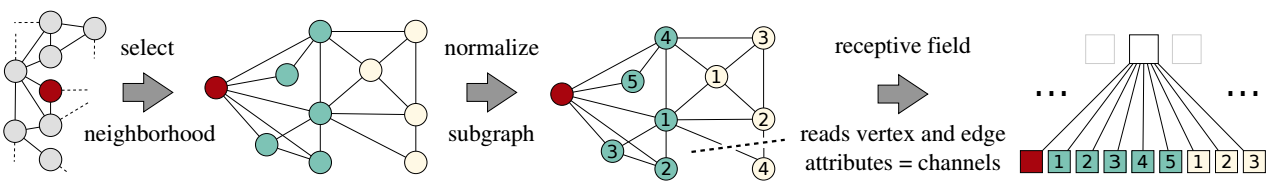
\includegraphics[width=.9\textwidth]{images/normalization}
\end{figure}
